\section{\ac{SMT}-solvers}

\subsection{School-level system of equations}

I've got this school-level system of equations copypasted from Wikipedia
\footnote{\url{https://en.wikipedia.org/wiki/System_of_linear_equations}}:

\begin{alignat*}{7}
3x &&\; + \;&& 2y             &&\; - \;&& z  &&\; = \;&& 1 & \\
2x &&\; - \;&& 2y             &&\; + \;&& 4z &&\; = \;&& -2 & \\
-x &&\; + \;&& \tfrac{1}{2} y &&\; - \;&& z  &&\; = \;&& 0 &
\end{alignat*}

Will it be possible to solve it using Z3? Here it is:

\begin{lstlisting}
#!/usr/bin/python
from z3 import *

x = Real('x')
y = Real('y')
z = Real('z')
s = Solver()
s.add(3*x + 2*y - z == 1)
s.add(2*x - 2*y + 4*z == -2)
s.add(-x + 0.5*y - z == 0)
print s.check()
print s.model()
\end{lstlisting}

We see this after run:

\begin{lstlisting}
sat
[z = -2, y = -2, x = 1]
\end{lstlisting}

If we change any equation in some way so it will have no solution, s.check() will return ``unsat''.

I've used ``Real'' \textit{sort} (some kind of data type in \ac{SMT}-solvers)
because the last expression equals to $\frac{1}{2}$, which is, of course, a real number.
For the integer system of equations, ``Int'' \textit{sort} would work fine.

Python (and other high-level \ac{PL}s like C\#) interface is highly popular, because it's practical, but in fact, 
there is a standard language for \ac{SMT}-solvers called SMT-LIB
\footnote{\url{http://smtlib.cs.uiowa.edu/papers/smt-lib-reference-v2.5-r2015-06-28.pdf}}.

Our example rewritten to it looks like this:

\begin{lstlisting}
(declare-const x Real)
(declare-const y Real)
(declare-const z Real)
(assert (=(-(+(* 3 x) (* 2 y)) z) 1))
(assert (=(+(-(* 2 x) (* 2 y)) (* 4 z)) -2))
(assert (=(-(+ (- 0 x) (* 0.5 y)) z) 0))
(check-sat)
(get-model)
\end{lstlisting}

This language is very close to LISP, but is somewhat hard to read for untrained eyes.

Now we run it:

\begin{lstlisting}
% z3 -smt2 example.smt
sat
(model
  (define-fun z () Real
    (- 2.0))
  (define-fun y () Real
    (- 2.0))
  (define-fun x () Real
    1.0)
)
\end{lstlisting}

So when you look back to my Python code, you may feel that these 3 expressions could be executed.
This is not true: Z3Py API offers overloaded operators, so expressions are constructed and passed into the guts of Z3 without any execution
\footnote{\url{https://github.com/Z3Prover/z3/blob/6e852762baf568af2aad1e35019fdf41189e4e12/src/api/python/z3.py}}.
I would call it ``embedded \ac{DSL}''.

Same thing for Z3 C++ API, you may find there ``operator+'' declarations and many more
\footnote{\url{https://github.com/Z3Prover/z3/blob/6e852762baf568af2aad1e35019fdf41189e4e12/src/api/c\%2B\%2B/z3\%2B\%2B.h}}.

Z3 \ac{API}s for Java, ML and .NET are also exist
\footnote{\url{https://github.com/Z3Prover/z3/tree/6e852762baf568af2aad1e35019fdf41189e4e12/src/api}}.\\
\\
Z3Py tutorial: \url{https://github.com/ericpony/z3py-tutorial}.

Z3 tutorial which uses SMT-LIB language: \url{http://rise4fun.com/Z3/tutorial/guide}.

\subsection{Another school-level system of equations}
\label{eq2_SMT}

I've found this somewhere at Facebook:

\begin{figure}[H]
\centering
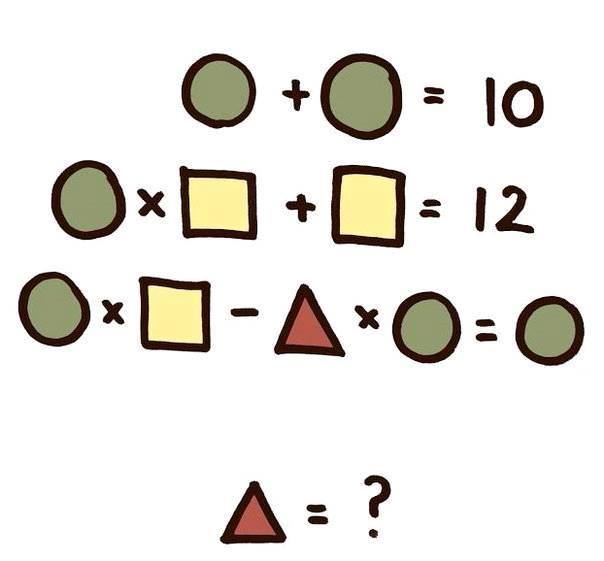
\includegraphics[scale=0.3]{SMT/equation.jpg}
\caption{System of equations}
\end{figure}

It's that easy to solve it in Z3:

\begin{lstlisting}
#!/usr/bin/python
from z3 import *

circle, square, triangle = Ints('circle square triangle')
s = Solver()
s.add(circle+circle==10)
s.add(circle*square+square==12)
s.add(circle*square-triangle*circle==circle)
print s.check()
print s.model()
\end{lstlisting}

\begin{lstlisting}
sat
[triangle = 1, square = 2, circle = 5]
\end{lstlisting}

\subsection{Connection between \ac{SAT} and \ac{SMT} solvers}

\ac{SMT}-solvers are frontends to \ac{SAT} solvers, i.e.,
they translating input SMT expressions into \ac{CNF} and feed SAT-solver with it.
Translation process is sometimes called ``bit blasting''.
Some \ac{SMT}-solvers uses external SAT-solver: STP uses MiniSAT or CryptoMiniSAT as backend.
Some other \ac{SMT}-solvers (like Z3) has their own SAT solver.

% subsections
\subsection{De Bruijn sequences; leading/trailing zero bits counting}

\subsubsection{Introduction}

Let's imagine there is a very simplified code lock accepting 2 digits, but it has no "enter" key, it just checks 2 last entered digits.
Our task is to brute force each 2-digit combination.
Naïve method is to try 00, 01, 02 ... 99.
That require 2*100=200 key pressings.
Will it be possible to reduce number of key pressings during brute-force?
It is indeed so, with the help of De Bruijn sequences.
We can generate them for the code lock, using Wolfram Mathematica:

\begin{lstlisting}
In[]:= DeBruijnSequence[{0, 1, 2, 3, 4, 5, 6, 7, 8, 9}, 2]
Out[]= {6, 8, 6, 5, 4, 3, 2, 1, 7, 8, 7, 1, 1, 0, 9, 0, 8, 0, 6, 6, \
0, 5, 5, 0, 4, 4, 0, 3, 3, 0, 2, 7, 2, 2, 0, 7, 7, 9, 8, 8, 9, 9, 7, \
0, 0, 1, 9, 1, 8, 1, 6, 1, 5, 1, 4, 1, 3, 7, 3, 1, 2, 9, 2, 8, 2, 6, \
2, 5, 2, 4, 7, 4, 2, 3, 9, 3, 8, 3, 6, 3, 5, 7, 5, 3, 4, 9, 4, 8, 4, \
6, 7, 6, 4, 5, 9, 5, 8, 5, 6, 9}
\end{lstlisting}

The result has exactly 100 digits, which is 2 times less than our initial idea can offer.
By scanning visually this 100-digits array, you'll find any number in 00..99 range.
All numbers are overlapped with each other: second half of each number is also first half of the next number, etc.

Here is another. We need a sequence of binary bits with all 3-bit numbers in it:

\begin{lstlisting}
In[]:= DeBruijnSequence[{0, 1}, 3]
Out[]= {1, 0, 1, 0, 0, 0, 1, 1}
\end{lstlisting}

Sequence length is just 8 bits, but it has all binary numbers in 000..111 range.
You may visually spot 000 in the middle of sequence.
111 is also present: two first bits of it at the end of sequence and the last bit is in the beginning.
This is so because De Bruijn sequences are cyclic.

There is also visual demonstration: \url{http://demonstrations.wolfram.com/DeBruijnSequences/}.

\subsubsection{Trailing zero bits counting}

In \href{https://en.wikipedia.org/wiki/De_Bruijn_sequence}{the Wikipedia article about De Bruijn sequences} we can find:

\begin{framed}
\begin{quotation}
The symbols of a De Bruijn sequence written around a circular object (such as a wheel of a robot) can be used to identify its angle by examining the n consecutive symbols facing a fixed point.
\end{quotation}
\end{framed}

Indeed: if we know De Bruijn sequence and we observe only part of it (any part), we can deduce exact position of this part within sequence.

Let's see, how this feature can be used.

Let's say, there is a need to detect position of input bit within 32-bit word.
For 0x1, the algorithm should report 1.
2 for 0x2.
3 for 0x4.
And 31 for 0x80000000.

The result is in 0..31 range, so the result can be stored in 5 bits.

We can construct binary De Bruijn sequence for all 5-bit numbers:

\begin{lstlisting}
In[]:= tmp = DeBruijnSequence[{0, 1}, 5]
Out[]= {1, 1, 1, 0, 0, 1, 1, 0, 1, 0, 1, 1, 1, 1, 1, 0, 1, 1, 0, 0, 0, 1, 0, 1, 0, 0, 1, 0, 0, 0, 0, 0}

In[]:= BaseForm[FromDigits[tmp, 2], 16]
Out[]:= e6bec520
\end{lstlisting}

Let's also recall that division some number by $2^n$ number is the same thing as shifting it by $n$ bits.
So if you divide 0xe6bec520 by 1, the result is not shifted, it is still the same.
If if divide 0xe6bec520 by 4 ($2^2$), the result is shifted by 2 bits.
We then take result and isolate lowest 5 bits.
This result is unique number for each input.
Let's shift 0xe6bec520 by all possible count number, and we'll get all possible last 5-bit values:

\begin{lstlisting}
In[]:= Table[BitAnd[BitShiftRight[FromDigits[tmp, 2], i], 31], {i, 0, 31}]
Out[]= {0, 16, 8, 4, 18, 9, 20, 10, 5, 2, 17, 24, 12, 22, 27, 29, \
30, 31, 15, 23, 11, 21, 26, 13, 6, 19, 25, 28, 14, 7, 3, 1}
\end{lstlisting}

The table has no duplicates:

\begin{lstlisting}
In[]:= DuplicateFreeQ[%]
Out[]= True
\end{lstlisting}

Using this table, it's easy to build a \textit{magic} table.
OK, now working C example:

\begin{lstlisting}[style=customc]
#include <stdint.h>
#include <stdio.h>

int magic_tbl[32];

// returns single bit position counting from LSB
// not working for i==0
int bitpos (uint32_t i)
{
	return magic_tbl[(0xe6bec520/i) & 0x1F];
};

int main()
{
	// construct magic table
	// may be omitted in production code
	for (int i=0; i<32; i++)
		magic_tbl[(0xe6bec520/(1<<i)) & 0x1F]=i;

	// test
	for (int i=0; i<32; i++)
	{
		printf ("input=0x%x, result=%d\n", 1<<i, bitpos (1<<i));
	};
};
\end{lstlisting}

Here we feed our bitpos() function with numbers in 0..0x80000000 range and we got:

\begin{lstlisting}
input=0x1, result=0
input=0x2, result=1
input=0x4, result=2
input=0x8, result=3
input=0x10, result=4
input=0x20, result=5
input=0x40, result=6
input=0x80, result=7
input=0x100, result=8
input=0x200, result=9
input=0x400, result=10
input=0x800, result=11
input=0x1000, result=12
input=0x2000, result=13
input=0x4000, result=14
input=0x8000, result=15
input=0x10000, result=16
input=0x20000, result=17
input=0x40000, result=18
input=0x80000, result=19
input=0x100000, result=20
input=0x200000, result=21
input=0x400000, result=22
input=0x800000, result=23
input=0x1000000, result=24
input=0x2000000, result=25
input=0x4000000, result=26
input=0x8000000, result=27
input=0x10000000, result=28
input=0x20000000, result=29
input=0x40000000, result=30
input=0x80000000, result=31
\end{lstlisting}

The bitpos() function actually counts trailing zero bits, but it works only for input values where only one bit is set.
To make it more practical, we need to devise a method to drop all leading bits except of the last one.
This method is very simple and well-known:

\begin{lstlisting}
input & (-input)
\end{lstlisting}

This bit twiddling hack can solve the job. Feeding 0x11 to it, it will return 0x1. Feeding 0xFFFF0000, it will return 0x10000.
In other words, it leaves lowest significant bit of the value, dropping all others.

It works because negated value in two's complement environment is the value with all bits flipped but also 1 added (because there is a zero in the middle of ring).
For example, let's take 0xF0. -0xF0 is 0x10 or 0xFFFFFF10. ANDing 0xF0 and 0xFFFFFF10 will produce 0x10.

Let's modify our algorithm to support true trailing zero bits count:

\begin{lstlisting}[style=customc]
#include <stdint.h>
#include <stdio.h>

int magic_tbl[32];

// not working for i==0
int tzcnt (uint32_t i)
{
	uint32_t a=i & (-i);
	return magic_tbl[(0xe6bec520/a) & 0x1F];
};

int main()
{
	// construct magic table
	// may be omitted in production code
	for (int i=0; i<32; i++)
		magic_tbl[(0xe6bec520/(1<<i)) & 0x1F]=i;

	// test:
	printf ("%d\n", tzcnt (0xFFFF0000));
	printf ("%d\n", tzcnt (0xFFFF0010));
};
\end{lstlisting}

It works!

\begin{lstlisting}
16
4
\end{lstlisting}

But it has one drawback: it uses division, which is slow.
Can we just multiplicate De Bruijn sequence by the value with the bit isolated instead of dividing sequence?
Yes, indeed.
Let's check in Mathematica:

\begin{lstlisting}
In[]:= BaseForm[16^^e6bec520*16^^80000000, 16]
Out[]:= 0x735f629000000000
\end{lstlisting}

The result is just too big to fit in 32-bit register, but can be used.
MUL/IMUL instruction 32-bit x86 CPUs stores 64-bit result into two 32-bit registers pair, yes.
But let's suppose we would like to make portable code which will work on any 32-bit architecture.
First, let's again take a look on De Bruijn sequence Mathematica first produced:

\begin{lstlisting}
In[]:= tmp = DeBruijnSequence[{0, 1}, 5]
Out[]= {1, 1, 1, 0, 0, 1, 1, 0, 1, 0, 1, 1, 1, 1, 1, 0, 1, 1, 0, 0, \
0, 1, 0, 1, 0, 0, 1, 0, 0, 0, 0, 0}
\end{lstlisting}

There is exactly 5 bits at the end which can be dropped.
The "magic" constant will be much smaller:

\begin{lstlisting}
In[]:= BaseForm[BitShiftRight[FromDigits[tmp, 2], 5], 16]
Out[]:=0x735f629
\end{lstlisting}

The "magic" constant is now "divided by 32 (or 1>>5)".
This mean that the result of multiplication of some value with one isolated bit by new magic number will also be smaller, so the bits we need will
be stored at the high 5 bits of the result.

De Bruijn sequence is not broken after 5 lowest bits dropped, because these zero bits are "relocated" to the start of the sequence.
Sequence is cyclic after all.

\begin{lstlisting}[style=customc]
#include <stdint.h>
#include <stdio.h>

int magic_tbl[32];

// not working for i==0
int tzcnt (uint32_t i)
{
	uint32_t a=i & (-i);
	// 5 bits we need are stored in 31..27 bits of product, shift and isolate them after multiplication:
	return magic_tbl[((0x735f629*a)>>27) & 0x1F];
};

int main()
{
	// construct magic table
	// may be omitted in production code
	for (int i=0; i<32; i++)
		magic_tbl[(0x735f629<<i >>27) & 0x1F]=i;
	
	// test:
	printf ("%d\n", tzcnt (0xFFFF0000));
	printf ("%d\n", tzcnt (0xFFFF0010));
};
\end{lstlisting}

\subsubsection{Leading zero bits counting}

This is almost the same task, but most significant bit must be isolated instead of lowest.
This is typical algorithm for 32-bit integer values:

\begin{lstlisting}
x |= x >> 1;
x |= x >> 2;
x |= x >> 4;
x |= x >> 8;
x |= x >> 16;
\end{lstlisting}

For example, 0x100 becomes 0x1ff, 0x1000 becomes 0x1fff, 0x20000 becomes 0x3ffff, 0x12340000 becomes 0x1fffffff.
It works because all 1 bits are gradually propagated towards the lowest bit in 32-bit number,
while zero bits at the left of most significant 1 bit are not touched.

It's possible to add 1 to resulting number, so it will becomes 0x2000 or 0x20000000, but in fact, since multiplication by magic number is used,
these numbers are very close to each other, so there are no error.

% FIXME URL
This example I used in my reverse engineering exercise from 15-Aug-2015: \url{https://yurichev.com/blog/2015-aug-18/}.

\begin{lstlisting}
int v[64]=
	{ -1,31, 8,30, -1, 7,-1,-1, 29,-1,26, 6, -1,-1, 2,-1,
	  -1,28,-1,-1, -1,19,25,-1, 5,-1,17,-1, 23,14, 1,-1,
	   9,-1,-1,-1, 27,-1, 3,-1, -1,-1,20,-1, 18,24,15,10,
	  -1,-1, 4,-1, 21,-1,16,11, -1,22,-1,12, 13,-1, 0,-1 };

int LZCNT(uint32_t x)
{
    x |= x >> 1;
    x |= x >> 2;
    x |= x >> 4;
    x |= x >> 8;
    x |= x >> 16;
    x *= 0x4badf0d;
    return v[x >> 26];
}
\end{lstlisting}

This piece of code I took from \href{http://stackoverflow.com/questions/7365562/de-bruijn-like-sequence-for-2n-1-how-is-it-constructed/7369288#7369288}{here}.
It is slightly different: the table is twice bigger, and the function returns -1 if input value is zero.
The magic number I found using just brute-force, so the readers will not be able to google it, for the sake of exercise.
(By the way, I've got 12,665,720 magic numbers which can serve this purpose.
This is about 0.294% of all 32-bit numbers.)

The code is tricky after all, and the moral of the exercise is that practicing reverse engineer sometimes may just observe input/outputs to understand
code's behaviour instead of diving into it.

\subsubsection{Performance}

The algorithms considered are probably fastest known, they has no conditional jumps, which is very good for CPUs starting at RISCs.
Newer CPUs has LZCNT and TZCNT instructions, even 80386 had BSF/BSR instructions which can be used for this: 
\url{https://en.wikipedia.org/wiki/Find_first_set}.
Nevertheless, these algorithms can be still used on cheaper RISC CPUs without specialized instructions.

\subsubsection{Applications}

Number of leading zero bits is binary logarithm of value. My article about logarithms including binary:
\url{https://yurichev.com/writings/log_intro.pdf}.

These algorithms are also extensively used in chess engines programming, where each piece is represented as 64-bit bitmask (chess board has 64 squares):
\url{http://chessprogramming.wikispaces.com/BitScan}.

There are more: \url{https://en.wikipedia.org/wiki/Find_first_set\#Applications}.

\subsubsection{Generation of De Bruijn sequences}

De Bruijn graph is a graph where all values are represented as vertices (or nodes) and each edge (or link) connects two nodes which can be "overlapped".
Then we need to visit each edge only once, this is called \textit{eulerian path}.
It is like the famous \textit{task of seven bridges of Königsberg}:
traveller must visit each bridge only once.

There are also simpler algorithms exist: \url{https://en.wikipedia.org/wiki/De_Bruijn_sequence\#Algorithm}.

\subsubsection{Other articles}

At least these are worth reading:
\url{http://supertech.csail.mit.edu/papers/debruijn.pdf},
\url{http://alexandria.tue.nl/repository/books/252901.pdf},
\href{https://en.wikipedia.org/wiki/De_Bruijn_sequence}{Wikipedia Article about De Bruijn sequences}.


\subsection{Generating de Bruijn sequences using Z3}
\label{DeBruijnZ3}

The following piece of quite esoteric code calculates number of leading zero bits
\footnote{\url{https://en.wikipedia.org/wiki/Find_first_set}}:

\begin{lstlisting}
int v[64]=
	{ -1,31, 8,30, -1, 7,-1,-1, 29,-1,26, 6, -1,-1, 2,-1,
	  -1,28,-1,-1, -1,19,25,-1, 5,-1,17,-1, 23,14, 1,-1,
	   9,-1,-1,-1, 27,-1, 3,-1, -1,-1,20,-1, 18,24,15,10,
	  -1,-1, 4,-1, 21,-1,16,11, -1,22,-1,12, 13,-1, 0,-1 };

int LZCNT(uint32_t x)
{
    x |= x >> 1;
    x |= x >> 2;
    x |= x >> 4;
    x |= x >> 8;
    x |= x >> 16;
    x *= 0x4badf0d;
    return v[x >> 26];
}
\end{lstlisting}

(This is usually done using simpler algorithm, but it will contain conditional jumps, which is bad for
CPUs starting at RISC. There are no conditional jumps in this algorithm.)

Read more about it: \url{https://yurichev.com/blog/de_bruijn/}.
The magic number used here is called \textit{de Bruijn sequence},
and I once used bruteforce to find it (one of the results was \textit{0x4badf0d}, which is used here).
But what if we need magic number for 64-bit values?
Bruteforce is not an option here.

If you already read about these sequences in my blog or in other sources,
you can see that the 32-bit magic number is a number consisting
of 5-bit overlapping chunks, and all chunks must be unique, i.e., must not be repeating.

For 64-bit magic number, these are 6-bit overlapping chunks.

To find the magic number, one can find a Hamiltonian path of a de Bruijn graph.
But I've found that Z3 is also can do this, though, overkill, but this is more illustrative.

\lstinputlisting[style=custompy]{SMT/de_bruijn_SMT/64.py}

We just enumerate all overlapping 6-bit chunks and tell Z3 that they must be unique (see \TT{Distinct}).
Output:

\lstinputlisting{SMT/de_bruijn_SMT/output.txt}

Overlapping chunks are clearly visible.
So the magic number is \textit{0x79c52dd0991abf60}.
Let's check:

\lstinputlisting{SMT/de_bruijn_SMT/64.c}

That works!

More about de Bruijn sequences:
\url{https://chessprogramming.wikispaces.com/De+Bruijn+sequence},
\url{https://chessprogramming.wikispaces.com/De+Bruijn+Sequence+Generator}.


\subsection{Package manager and Z3}

Here is simplified example.
We have libA, libB, libC and libD, available in various versions (and flavors).
We're going to install programA and programB, which use these libraries.

\lstinputlisting{SMT/dep/dependency.py}

( The source code: \url{https://github.com/DennisYurichev/SAT_SMT_article/blob/master/SMT/dep/dependency.py} )

The output:

\begin{lstlisting}
sat
[libB = 5,
 libD = 999,
 libC = 10,
 programB = 7,
 programA = 1,
 libA = 2]
\end{lstlisting}

999 means that there is no need to install libD, it's not required by other packages.

Change version of ProgramB to v8 and it will says ``unsat'', meaning, there is a conflict:
ProgramA requires libA v2, but ProgramB v8 eventually requires newer libA.

Still, there is a work to do: ``unsat'' message is somewhat useless to end user,
some information about conflicting items should be printed.

Here is my another optimization problem example: \ref{set_cover}.

More about using SAT/SMT solvers in package managers: \url{https://research.swtch.com/version-sat},
\url{https://cseweb.ucsd.edu/~lerner/papers/opium.pdf}.

Now in the opposite direction: forcing aptitude package manager to solve Sudoku: \\
\url{http://web.archive.org/web/20160326062818/http://algebraicthunk.net/~dburrows/blog/entry/package-management-sudoku/}.

Some readers may ask, how to order libraries/programs/packages to be installed?
This is simpler problem, which is often solved by topological sorting.
The algorithm reorders graph in such a way so that vertices not depended on anything will be on the top of queue.
Next, there will be vertices dependend on vertices from the previous layer.
And so on.

\textit{make} UNIX utility does this while constructing order of items to be processed.
Even more: older \textit{make} utilities offloaded the job to the external utility (\textit{tsort}).
Some older UNIX has it, at least some versions of NetBSD
\footnote{\url{http://netbsd.gw.com/cgi-bin/man-cgi/man?tsort+1+NetBSD-current}}.


\subsection{Tiling puzzle and Z3 SMT solver}
\label{tiling_Z3}

This is classic problem: given 12 polyomino titles, cover mutilated chessboard with them (it has 60 squares with no central 4 squares).

The problem is covered at least in \href{https://arxiv.org/pdf/cs/0011047.pdf}{Donald E. Knuth - Dancing Links},
and this Z3 solution has been inspired by it.

Another thing I've added: graph coloring. You see, my script gives correct solutions, but somewhat unpleasant visually.
So I used colored pseudographics. There are 12 tiles, it's not a problem to assign 12 colors to them.
But there is another heavily used SAT problem: graph coloring.

Given a graph, assign a color to each vertex/node, so that colors wouldn't be equal in adjacent nodes.
The problem can be solved easily in SMT: assign variable to each vertex.
If two vertices are connected, add a constraint: \textit{vertex1\_color != vertex2\_color}.
As simple as that.
In my case, each polynomio is vertex and if polyomino is adjacent to another polyomino, an edge/link is added between vertices.
So I did, and output is now colored.

But this is planar graph (i.e., a graph which is, if represented in two-dimensional space has no intersected edges/links).
And here is a famous four color theorem can be used.
The solution of tiled polynomios is in fact like planar graph, or, a map, like a world map.
Theorem states that any planar graph (or map) can be colored only 4 colors.

This is true, even more, several tilings can be colors with only 3 colors:

\begin{figure}[H]
\centering
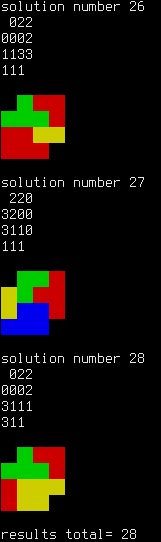
\includegraphics[scale=1]{SMT/tiling/small.png}
\caption{}
\end{figure}

Now the classic: 12 pentominos and "mutilated" chess board, several solutions:

% TODO side by side in table:
\begin{figure}[H]
\centering
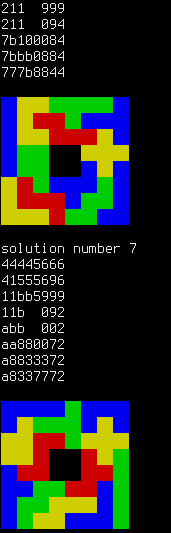
\includegraphics[scale=1]{SMT/tiling/big1.png}
\caption{}
\end{figure}

\begin{figure}[H]
\centering
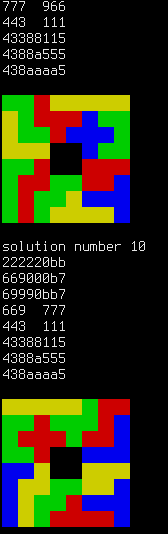
\includegraphics[scale=1]{SMT/tiling/big2.png}
\caption{}
\end{figure}

% FIXME URL
The source code: \url{.../tiling.py}.

Further reading: \url{https://en.wikipedia.org/wiki/Exact_cover#Pentomino_tiling}.

Four-color theorem has an interesting story, it has been finally proved in 2005 by Coq proof assistant:
\url{https://en.wikipedia.org/wiki/Four_color_theorem}.


\subsection{Ménage problem}

\begin{lstlisting}
In combinatorial mathematics, the ménage problem or problème des ménages[1] asks for the number of different ways in which it is possible to seat a set of male-female couples at a dining table so that men and women alternate and nobody sits next to his or her partner. This problem was formulated in 1891 by Édouard Lucas and independently, a few years earlier, by Peter Guthrie Tait in connection with knot theory.[2] For a number of couples equal to 3, 4, 5, ...  the number of seating arrangements is

    12, 96, 3120, 115200, 5836320, 382072320, 31488549120, ... (sequence A059375 in the OEIS). 
\end{lstlisting}

( \href{https://en.wikipedia.org/wiki/M%C3%A9nage_problem}{Wikipedia}. )

We can count it using Z3, but also get actual men/women allocations:

\lstinputlisting{SMT/menage.py}

( \url{URL} )

For 3 couples:

\begin{lstlisting}
  men 0 2 1
women  1 0 2

  men 1 2 0
women  0 1 2

  men 0 1 2
women  2 0 1

  men 2 1 0
women  0 2 1

  men 2 0 1
women  1 2 0

  men 1 0 2
women  2 1 0

results total= 6
however, according to https://oeis.org/A059375 : 12
\end{lstlisting}

We are getting ``half'' of results because men and women can be then swapped (their sex swapped (or reassigned))
and you've got another 6 results.
6+6=12 in total.
This is kind of symmetry.

For 4 couples:

\begin{lstlisting}

...

  men 3 0 2 1
women  1 3 0 2

  men 3 0 1 2
women  2 3 0 1

  men 1 0 2 3
women  3 1 0 2

  men 2 0 1 3
women  3 2 0 1

results total= 48
however, according to https://oeis.org/A059375 : 96
\end{lstlisting}

For 5 couples:

\begin{lstlisting}

...

  men 0 4 1 2 3
women  1 3 0 4 2

  men 0 3 1 2 4
women  1 4 0 3 2

  men 0 3 1 2 4
women  1 0 4 3 2

  men 4 3 1 0 2
women  0 2 4 1 3

results total= 1560
however, according to https://oeis.org/A059375 : 3120
\end{lstlisting}


\subsection{Stable marriage problem}

See also in
\href{https://en.wikipedia.org/wiki/Stable_marriage_problem}{Wikipedia} and 
\href{https://rosettacode.org/wiki/Stable_marriage_problem}{Rosetta code}.

Layman's explanation in Russian: \url{https://lenta.ru/articles/2012/10/15/nobel/}.

My solution is much less efficient, because much simpler/better algorithm exists (Gale/Shapley algorithm),
but I did it to demonstrate the essence of the problem plus as a yet another SMT-solvers and Z3 demonstration.

See comments:

\lstinputlisting{SMT/stable_marriage/stable.py}

( The source code: \url{URL/stable.py} )

Result is seems to be correct:

\begin{lstlisting}
sat

ManChoice:
abe <-> ivy
bob <-> cath
col <-> dee
dan <-> fay
ed <-> jan
fred <-> bea
gav <-> gay
hal <-> eve
ian <-> hope
jon <-> abi

WomanChoice:
abi <-> jon
bea <-> fred
cath <-> bob
dee <-> col
eve <-> hal
fay <-> dan
gay <-> gav
hope <-> ian
ivy <-> abe
jan <-> ed
\end{lstlisting}

This is what we did in plain English language.
``Connect men and women somehow, we don't care how.
But no pair must exist of those who prefer each other (simultaneously) over their current spouses''.
Gale/Shapley algorithm uses ``steps'' to ``stabilize'' marriage.
There are no ``steps'', all pairs are married couples already.

Another important thing to notice: only one solution must exist.

\begin{lstlisting}
...

results=[]

# enumerate all possible solutions:
while True:
    if s.check() == sat:
        m = s.model()
        #print m
        results.append(m)
        block = []
        for d in m:
            c=d()
            block.append(c != m[d])
        s.add(Or(block))
    else:
        print "results total=", len(results)
        break

...
\end{lstlisting}

( The source code: \url{URL/stable2.py} )

That reports only 1 model available, which is correct indeed.


\subsection{Dependency graphs and topological sorting}

Topological sorting is an operation many programmers well familiar with: this is what ``make'' tool
do when it find an order of items to process.
Items not dependent of anything can be processed first.
The most dependent items at the end.

Dependency graph is a graph and topological sorting is such a ``contortion'' of the a graph,
when you can see an order of items.

For example, let's create a sample graph in Wolfram Mathematica:

\begin{lstlisting}
In[]:= g = Graph[{7 -> 1, 7 -> 0, 5 -> 1, 3 -> 0, 3 -> 4, 1 -> 2, 1 -> 6, 
   1 -> 4, 0 -> 6}, VertexLabels -> "Name"]
\end{lstlisting}

\begin{figure}[H]
\centering
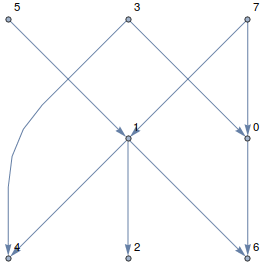
\includegraphics[scale=0.6]{SMT/tsort/math.png}
\caption{}
\end{figure}

Each arrow shows that an item is needed by an item arrow pointing to, i.e., if ``a -> b'', then item ``a'' must be first
processed, because ``b'' needs it, or ``b'' depends on ``a''.

How Mathematica would ``sort'' the dependency graph?

\begin{lstlisting}
In[]:= TopologicalSort[g]
Out[]= {7, 3, 0, 5, 1, 4, 6, 2}
\end{lstlisting}

So you're going to process item 7, then 3, 0, and 2 at the very end.

\href{https://en.wikipedia.org/wiki/Topological_sorting}{The algorithm in the Wikipedia article}
is probably used in the ``make'' and whatever IDE you use for building your code.

Also, many UNIX platforms had separate ``tsort'' utility:
\url{https://en.wikipedia.org/wiki/Tsort}.

How would ``tsort'' sort the graph? I'm making the text file with input data:

\begin{lstlisting}
7 1
7 0
5 1
3 0
3 4
1 2
1 6
1 4
0 6
\end{lstlisting}

And run tsort:

\begin{lstlisting}
 % tsort tst
3
5
7
0
1
4
6
2
\end{lstlisting}

Now I'll use Z3 SMT-solver for topological sort, which is overkill, but quite spectacular: all we need to do
is to add constraint for each edge (or ``connection'') in graph, if ``a -> b'', then ``a'' must be less then ``b'', where
each variable reflects ordering.

\lstinputlisting{SMT/tsort/tsort.py}

Almost the same result, but also correct:

\begin{lstlisting}
sat
[3, 5, 7, 0, 1, 2, 4, 6]
\end{lstlisting}


\subsection{Travelling salesman problem}

This is it:

\lstinputlisting{SMT/TSP/TSP.py}

The result:

\begin{lstlisting}
sat
Dallas (1240 mi to the next city) ->
Los Angeles (831 mi to the next city) ->
Denver (700 mi to the next city) ->
Minneapolis (355 mi to the next city) ->
Chicago (713 mi to the next city) ->
New York (1374 mi to the next city) ->
distance_total= 5213 mi
\end{lstlisting}

Map I generated with Wolfram Mathematica:

\begin{figure}[H]
\centering
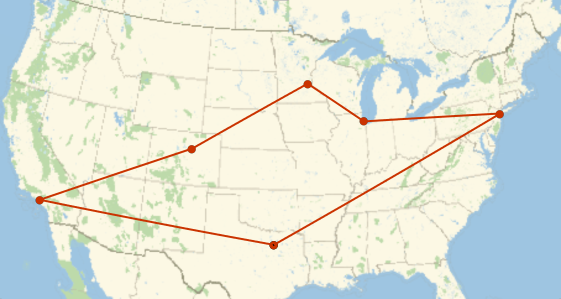
\includegraphics[scale=0.6]{SMT/TSP/map1.png}
\caption{}
\end{figure}

Maximizing:

\begin{lstlisting}
sat
Dallas (862 mi to the next city) ->
Minneapolis (700 mi to the next city) ->
Denver (1631 mi to the next city) ->
New York (2451 mi to the next city) ->
Los Angeles (1745 mi to the next city) ->
Chicago (803 mi to the next city) ->
distance_total= 8192 mi
\end{lstlisting}

The map:

\begin{figure}[H]
\centering
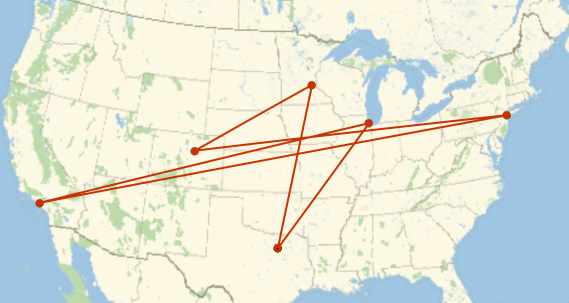
\includegraphics[scale=0.6]{SMT/TSP/map2.png}
\caption{}
\end{figure}

I could only process 6 cities, and it takes starting at several seconds up to 1 minute on my venerable Intel Quad-Core Xeon E3-1220 3.10GHz.
Perhaps, this is not a right tool for the job, well-known TSP algorithms way faster.

Even bruteforce enumeration is way faster ($6!=720$ paths).

However, it still can serve as demonstration.


\subsection{Crossword generator}

We assign an integer to each character in crossword, it reflects ASCII code of it.

Then we enumerate all possible horizontal/vertical ``sticks'' longer than 1 and assign words to them.

For example, there is a horizontal stick of length 3.
And we have such 3-letter words in our dictionary: ``the'', ``she'', ``xor''.

We add the following constraint:

\begin{lstlisting}
Or(
	And(chars[X][Y]=='t', chars[X][Y+1]=='h', chars[X][Y+2]=='e'),
	And(chars[X][Y]=='s', chars[X][Y+1]=='h', chars[X][Y+2]=='e'),
	And(chars[X][Y]=='x', chars[X][Y+1]=='o', chars[X][Y+2]=='r'))
\end{lstlisting}

One of these words would be choosen automatically.

Index of each word is also considered, because duplicates are not allowed.

Sample pattern:

\begin{lstlisting}
**** **********
 * * *  * * * *
***************
 * * *  * * * *
********* *****
 * * * * * *  *
****** ********
   * * * * *   
******** ******
*  * * * * * * 
***** *********
* * * *  * * * 
***************
* * * *  * * * 
********** ****
\end{lstlisting}

Sample result:

\begin{lstlisting}
spur stimulated
 r e c  i a h e
congratulations
 m u t  a i s c
violation niece
 s a e p e n  n
rector penitent
   i i o c e
accounts herald
s  n g e a r o
press edinburgh
e x e n  t p i
characteristics
t c l r  n e a
satisfying dull

horizontal:
((0, 0), (0, 3)) spur
((0, 5), (0, 14)) stimulated
((2, 0), (2, 14)) congratulations
((4, 0), (4, 8)) violation
((4, 10), (4, 14)) niece
((6, 0), (6, 5)) rector
((6, 7), (6, 14)) penitent
((8, 0), (8, 7)) accounts
((8, 9), (8, 14)) herald
((10, 0), (10, 4)) press
((10, 6), (10, 14)) edinburgh
((12, 0), (12, 14)) characteristics
((14, 0), (14, 9)) satisfying
((14, 11), (14, 14)) dull
vertical:
((8, 0), (14, 0)) aspects
((0, 1), (6, 1)) promise
((10, 2), (14, 2)) exact
((0, 3), (10, 3)) regulations
((10, 4), (14, 4)) seals
((0, 5), (9, 5)) scattering
((10, 6), (14, 6)) entry
((4, 7), (10, 7)) opposed
((0, 8), (4, 8)) milan
((5, 9), (14, 9)) enchanting
((0, 10), (4, 10)) latin
((4, 11), (14, 11)) interrupted
((0, 12), (4, 12)) those
((8, 13), (14, 13)) logical
((0, 14), (6, 14)) descent
\end{lstlisting}

Unsat is possible if the dictionary is too small or have no words of length present in pattern.

The source code:

\lstinputlisting{SMT/cross/cross_Z3.py}

The files, including my dictionary: \url{https://github.com/DennisYurichev/yurichev.com...}.


\subsection{Exercise 15 from TAOCP ``7.1.3 Bitwise tricks and techniques''}

Page 53 from the fasc1a.ps, or: \url{http://www.cs.utsa.edu/~wagner/knuth/fasc1a.pdf}

\begin{figure}[H]
\label{fig:pipe_shuffled}
\centering
\frame{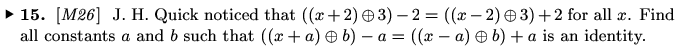
\includegraphics[scale=0.6]{SMT/TAOCP_7_1_3_exercise_15/page53.png}}
\caption{Page 53}
\end{figure}

Soltuion:

\begin{lstlisting}
from z3 import *

s=Solver()

a, b=BitVecs('a b', 4)
x, y=BitVecs('x y', 4)

s.add(ForAll(x, ForAll(y,  ((x+a)^b)-a == ((x-a)^b)+a  )))

# enumerate all possible solutions:
results=[]
while True:
    if s.check() == sat:
        m = s.model()
        print m

        results.append(m)
        block = []
        for d in m:
            c=d()
            block.append(c != m[d])
        s.add(Or(block))
    else:
        print "results total=", len(results)
        break
\end{lstlisting}

For 4-bit bitvectors:

\begin{lstlisting}

...

[b = 7, a = 0]
[b = 6, a = 8]
[b = 7, a = 8]
[b = 6, a = 12]
[b = 7, a = 12]
[b = 12, a = 0]
[b = 13, a = 0]
[b = 12, a = 8]
[b = 13, a = 8]
[b = 12, a = 4]
[b = 13, a = 4]
[b = 12, a = 12]
[b = 13, a = 12]
[b = 14, a = 0]
[b = 15, a = 0]
[b = 14, a = 4]
[b = 15, a = 4]
[b = 14, a = 8]
[b = 15, a = 8]
[b = 14, a = 12]
[b = 15, a = 12]
results total= 128
\end{lstlisting}


\subsection{Anroid lock screen (9 dots) has 140240 possible ways to (un)lock it}

How would you count?

\begin{lstlisting}
from z3 import *

"""
1 2 3
4 5 6
7 8 9
"""

# where the next dot can be if the current dot is at $a$
# next dot can only be a neighbour
# here we define starlike connections between dots (as in Android lock screen)
# this is like switch() or multiplexer

# lines like these are also counted:
# * . .
# . . *
# . * .
def next_dot(a, b):
    return If(a==1, Or(b==2, b==4, b==5, b==6, b==8),
        If(a==2, Or(b==1, b==3, b==4, b==5, b==6, b==7, b==9),
        If(a==3, Or(b==2, b==5, b==6, b==4, b==8),
        If(a==4, Or(b==1, b==2, b==5, b==7, b==8, b==3, b==9),
        If(a==5, Or(b==1, b==2, b==3, b==4, b==6, b==7, b==8, b==9),
        If(a==6, Or(b==2, b==3, b==5, b==8, b==9, b==1, b==7),
        If(a==7, Or(b==4, b==5, b==8, b==2, b==6),
        If(a==8, Or(b==4, b==5, b==6, b==7, b==9, b==1, b==3),
        If(a==9, Or(b==5, b==6, b==8, b==4, b==2),
            False))))))))) # default

# if only non-diagonal lines between dots are allowed:
"""
def next_dot(a, b):
    return If(a==1, Or(b==2, b==4),
        If(a==2, Or(b==1, b==3, b==5),
        If(a==3, Or(b==2, b==6),
        If(a==4, Or(b==1, b==5, b==7),
        If(a==5, Or(b==2, b==4, b==6, b==8),
        If(a==6, Or(b==3, b==5, b==9),
        If(a==7, Or(b==4, b==8),
        If(a==8, Or(b==5, b==7, b==9),
        If(a==9, Or(b==6, b==8),
            False))))))))) # default
"""

# old version, hasn't counted lines like
# * . .
# . . *
# . * .

"""
def next_dot(a, b):
    return If(a==1, Or(b==2, b==4, b==5),
        If(a==2, Or(b==1, b==3, b==4, b==5, b==6),
        If(a==3, Or(b==2, b==5, b==6),
        If(a==4, Or(b==1, b==2, b==5, b==7, b==8),
        If(a==5, Or(b==1, b==2, b==3, b==4, b==6, b==7, b==8, b==9),
        If(a==6, Or(b==2, b==3, b==5, b==8, b==9),
        If(a==7, Or(b==4, b==5, b==8),
        If(a==8, Or(b==4, b==5, b==6, b==7, b==9),
        If(a==9, Or(b==5, b==6, b==8),
            False))))))))) # default
"""

def paths_for_length (LENGTH):
    s=Solver()

    path=[Int('path_%d' % i) for i in range(LENGTH)]

    # all elements of path must be distinct
    s.add(Distinct(path))

    # all elements in [1..9] range:
    for i in range(LENGTH):
        s.add(And(path[i]>=1, path[i]<=9))

    # next element of path is defined by next_dot() function, unless it's the last one:
    for i in range(LENGTH-1):
        s.add(next_dot(path[i], path[i+1]))

    results=[]

    # enumerate all possible solutions:
    while True:
        if s.check() == sat:
            m = s.model()
            tmp=[]
            for i in range(LENGTH):
                tmp.append(m[path[i]].as_long())
            #print m
            print "path", tmp
            # print visual representation:
            for k in [[1,2,3],[4,5,6],[7,8,9]]:
                for j in k:
                    if j in tmp:
                        print tmp.index(j)+1,
                    else:
                        print ".",
                print ""
            print ""
            results.append(m)
            block = []
            for d in m:
                c=d()
                block.append(c != m[d])
            s.add(Or(block))
        else:
            print "length=", LENGTH, "results total=", len(results)
            return len(results)

total=0
for l in range(2,10):
    total=total+paths_for_length(l)

print "total=", total
\end{lstlisting}

Sample paths of 7 elements:

\begin{lstlisting}
...

path [7, 5, 1, 4, 8, 6, 3]
3 . 7
4 2 6
1 5 .

path [9, 5, 7, 4, 8, 6, 3]
. . 7
4 2 6
3 5 1

path [9, 5, 1, 4, 8, 6, 3]
3 . 7
4 2 6
. 5 1

...
\end{lstlisting}

Each element of ``path'' is number of dot, like on phone's keypad:

\begin{lstlisting}
1 2 3
4 5 6
7 8 9
\end{lstlisting}

Numbers on $3 \cdot 3$ box represent a sequence: which dot is the 1st, 2nd, etc...

Of 9:

\begin{lstlisting}
...

path [7, 8, 9, 5, 4, 1, 2, 6, 3]
6 7 9
5 4 8
1 2 3

path [1, 4, 7, 5, 2, 3, 6, 9, 8]
1 5 6
2 4 7
3 9 8

path [9, 6, 8, 7, 4, 1, 5, 2, 3]
6 8 9
5 7 2
4 3 1

...
\end{lstlisting}

All possible paths: \url{FIXME/all.bz2}

Statistics:

\begin{lstlisting}
length= 2 results total= 56
length= 3 results total= 304
length= 4 results total= 1400
length= 5 results total= 5328
length= 6 results total= 16032
length= 7 results total= 35328
length= 8 results total= 49536
length= 9 results total= 32256
total= 140240
\end{lstlisting}

What if only non-diagonal lines would be allowed (which isn't a case of a real Android lock screen)?

\begin{lstlisting}
length= 2 results total= 24
length= 3 results total= 44
length= 4 results total= 80
length= 5 results total= 104
length= 6 results total= 128
length= 7 results total= 112
length= 8 results total= 112
length= 9 results total= 40
total= 644
\end{lstlisting}

Also, at first, when I published this note, lines like these weren't counted (but allowable on Andoird lock screen, as it was pointed out by @mztropics):

\begin{lstlisting}
* . .
. . *
. * .
\end{lstlisting}

And the [incorrect] statistics was like this:

\begin{lstlisting}
length= 2 results total= 40
length= 3 results total= 160
length= 4 results total= 496
length= 5 results total= 1208
length= 6 results total= 2240
length= 7 results total= 2984
length= 8 results total= 2384
length= 9 results total= 784
total= 10296
\end{lstlisting}

Now you can see, how drastically number of all possibilities can change, when you add $\approx 2$ more branches at each element of path.


\subsection{Knight's tour}

\lstinputlisting[style=custompy]{SMT/knight_tour/knight_tour_Z3.py}

Can find a closed knight's tour on 8*8 chess board for 150s on Intel Quad-Core Xeon E3-1220 3.10GHz:

\begin{lstlisting}
 0 57 44 41  2 39 12 29
43 46  1 58 11 30 23 38
56 63 42 45 40  3 28 13
47  8 59 10 31 24 37 22
60 55 62 51  4 27 14 25
 7 48  9 32 17 34 21 36
54 61 50  5 52 19 26 15
49  6 53 18 33 16 35 20
\end{lstlisting}

However, this is WAY slower than C implementation on Rosetta Code: \url{https://rosettacode.org/wiki/Knight%27s_tour#C}
... which uses Warnsdorf's rule: \url{https://en.wikipedia.org/wiki/Knight%27s_tour#Warnsdorff.27s_algorithm}.

Another program for Z3 for finding Hamiltonian cycle: \url{https://github.com/Z3Prover/z3/blob/master/examples/python/hamiltonian/hamiltonian.py}.
(Clever trick of using remainder.)


\subsection{Hilbert's 10th problem, Fermat’s last theorem and SMT solvers}

Hilbert's 10th problem states that you cannot devise an algorithm which can solve any diophantine equation over integers.
However, it's important to understand, that this is possible over fixed-size bitvectors.

Fermat's last theorem states that there are no integer solution(s) for $a^n + b^n = c^n$, for $n>=3$.

Let's prove it for n=3 and for a in 0..255 range:

\lstinputlisting[style=custompy]{SMT/Hilbert_10/fermat.py}

Z3 gives "unsat", meaning, it couldn't find any a/b/c.
However, this is possible to check even using brute-force search.

If to replace "BitVecs" by "Ints", Z3 would give "unknown":

\lstinputlisting[style=custompy]{SMT/Hilbert_10/fermat2.py}

In short: anything is decidable (you can build an algorithm which can solve equation or not) under fixed-size bitvectors.
Given enough computational power, you can solve such equations for big bit-vectors.
But this is not possible for integers or bit-vectors of any size.

Another interesting reading about this by Leonardo de Moura:
\url{https://stackoverflow.com/questions/13898175/how-does-z3-handle-non-linear-integer-arithmetic}.



\subsection{List of SMT-solvers}

\begin{itemize}

\item Yices\footnote{\url{http://yices.csl.sri.com/}}, created by Bruno Dutertre et al.

\item Z3\footnote{\url{https://github.com/Z3Prover/z3}},
created by Leonardo de Moura, Nikolaj Bjorner, Christoph M. Wintersteiger.

	Many examples here uses Python 3.x API for Z3.
	Here is how to install it in Ubuntu:

	\begin{lstlisting}
	sudo apt-get install python3-pip
	sudo pip3 install z3-solver
	\end{lstlisting}

\item STP\footnote{\url{https://github.com/stp/stp}}, used in KLEE.

\item CVC3/CVC4\footnote{\url{http://cvc4.stanford.edu/}}.

\item Boolector\footnote{\url{http://fmv.jku.at/boolector/}}, created by Aina Niemetz, Mathias Preiner and Armin Biere.

\item Alt-Ergo\footnote{\url{https://alt-ergo.ocamlpro.com/}}, used in Frama-C.

\item MathSAT\footnote{\url{http://mathsat.fbk.eu/}}. Created by Alberto Griggio, Alessandro Cimatti and Roberto Sebastiani.

\item veriT\footnote{\url{http://www.verit-solver.org/}}.
Created by David Déharbe, Pascal Fontaine, Haniel Barbosa.
Bitvectors are not supported.

\item MK85\footnote{\url{https://github.com/DennisYurichev/MK85}}. Created by Dennis Yurichev, as a toy-level bit-blaster.

\end{itemize}



